\chapter{Results and Discussions}
%%%%%%%%%%%%%%%%%%%%%%%%%%%%%%%%%%%%%%%%%%%%%%%%%%%%%%%%%%%%
%%%%%%%%%%%%%%%%%%%%  NEW SECTION   %%%%%%%%%%%%%%%%%%%%%%%%
%%%%%%%%%%%%%%%%%%%%%%%%%%%%%%%%%%%%%%%%%%%%%%%%%%%%%%%%%%%%
\setcounter{equation}{0}

\nomenclature{CAST}{Concatenation of Attention enhanced Spatial and Temporal features}
\nomenclature{TP}{True Positive}
\nomenclature{FP}{False Positive}
\nomenclature{TN}{True Negative}
\nomenclature{FN}{False Negative}
\nomenclature{XAI}{Explainable AI}

\section{Model's Prediction on Unseen Data}

\noindent The Figure \ref{fig:FightPred} and Figure \ref{fig:noFightPred} show the predictive power of the model when given by a .npy file as input, during this testing phase the layers like Batch Normalization and Dropout Layers will be off. The output(prediction) of the model will be an average of calculations of the input frames in the model, as the model goes on to attend all the frames to make a representation of the input file. 

\begin{figure}[htbp]
    \centering
    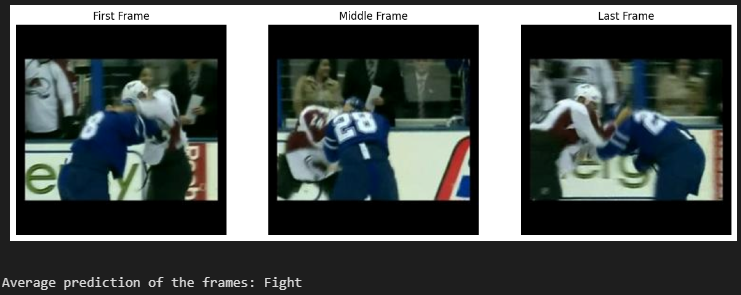
\includegraphics[width=1\textwidth]{Images/single_video_fight_pred.png}
    \caption{Model Prediction on a 'Fight' Video}
    \label{fig:FightPred}
\end{figure}

\begin{figure}[htbp]
    \centering
    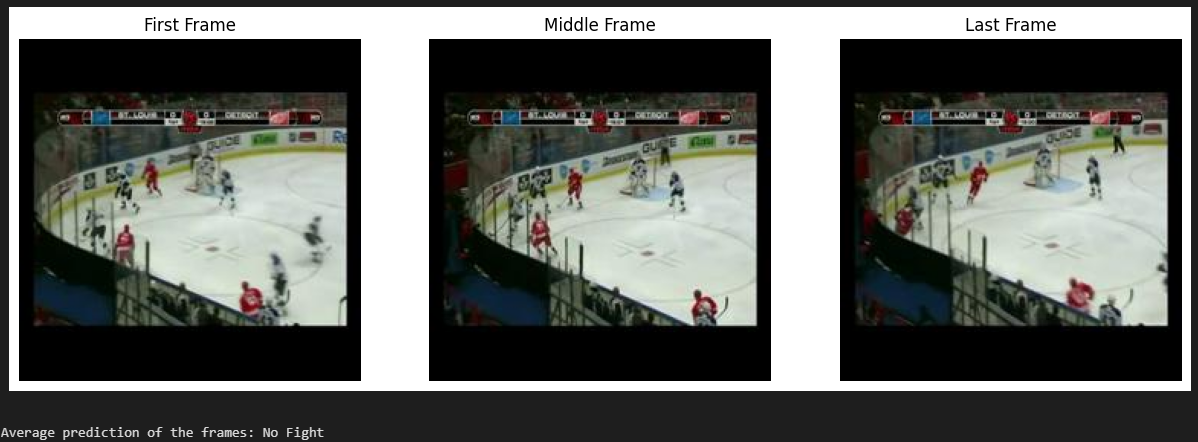
\includegraphics[width=1\textwidth]{Images/single_video_no_fight_pred.png}
    \caption{Model Prediction on a 'No-Fight' Video}
    \label{fig:noFightPred}
\end{figure}


\section{Performance Evaluation}

In this section, the performance of the proposed model is checked using various metrics to assess its effectiveness and reliability in achieving the intended outcomes. The primary objective of the project was to propose a lightweight system, that does not overfit on the data and trains in reasonable hardware resources. Though with the training most of these objectives were covered, there is a need to analyze the model in-depth to understand whether the model is robust, fast, and effective to unseen data.

\begin{itemize}
    \item Dataset Used: Hockey Fight Dataset

    \item Evaluation Metrics: Accuracy, Precision, Recall, and F1 Score.

    \item Testing methodology: The model will be tested on a separate part of the dataset called the testing set, which consists of 200 Videos under the labels Fight and No\_Fight.
\end{itemize}

% \begin{table}[htbp!]
% \centering
% \captionof{table}{Training and Testing Metrics}
% \begin{tabular}{c|c|c|c}
% \hline
% \textbf{Criteria} & \textbf{Metric} & \multicolumn{2}{c}{\textbf{Value (\%)}} \\
% \cline{3-4}
%            &                  & \textbf{Training}    & \textbf{Testing} \\ \hline
% Graph     & Accuracy          & 95.00                & 92.00               \\
% Testing   & Accuracy          & 89.00                   & 89.00                \\
% \hline
% \end{tabular}

% \label{table:trainingTestingAccMetric}
% \end{table}

\clearpage

\subsection{Accuracy-Loss Graph}

The Accuracy-Loss Graph is an essential visual tool that illustrates the model's performance across its training and validation phases. Accuracy measures the proportion of true results (both true positives and true negatives) among the total number of cases the model has gone through. Loss, on the other hand, quantifies the error between the predicted values and the actual values, which shows the model's precision during training. Therefore, these graphs help in understanding the model's learning curve and pinpointing any overfitting or underfitting issues.

\begin{figure}[htbp]
    \centering
    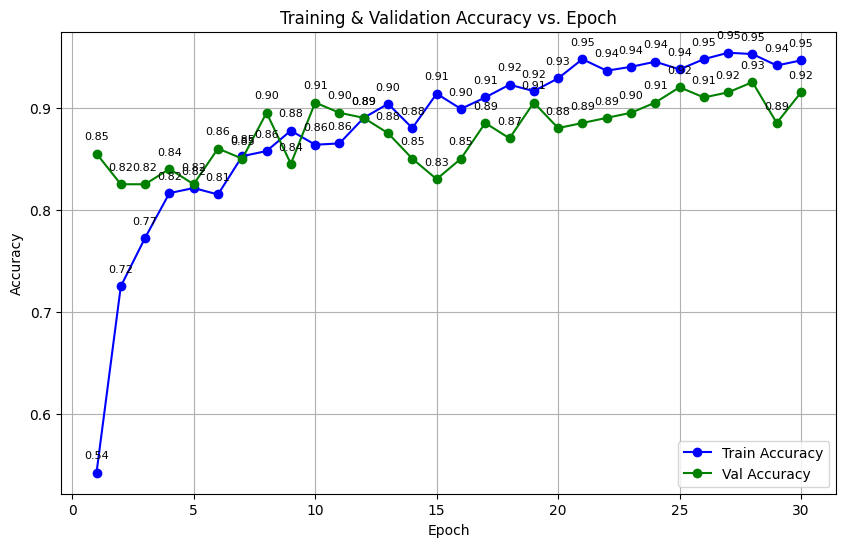
\includegraphics[width=1\textwidth]{Images/acc graph.png}
    \caption{Accuracy versus Epoch Graph}
    \label{fig:AccGraph}
\end{figure}

\begin{figure}[htbp]
    \centering
    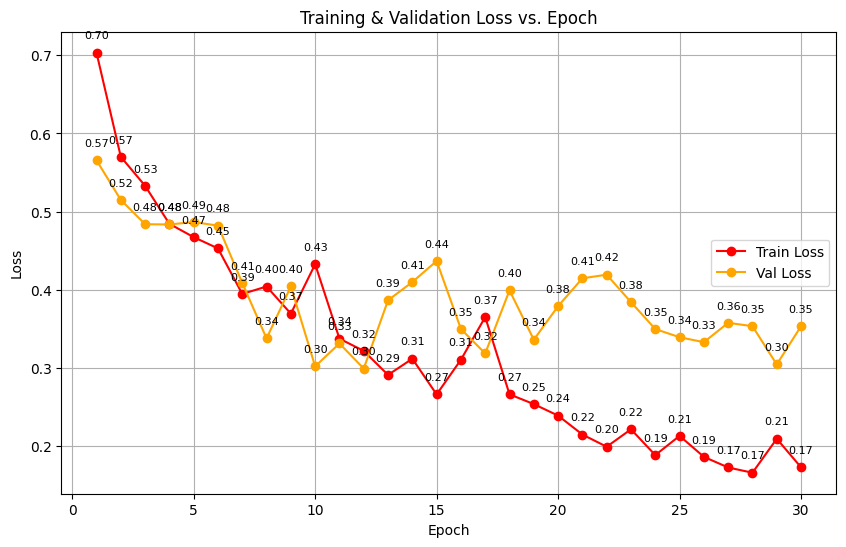
\includegraphics[width=1\textwidth]{Images/loss graph.png}
    \caption{Loss versus Epoch Graph}
    \label{fig:LossGraph}
\end{figure}

\begin{figure}[htbp]
    \centering
    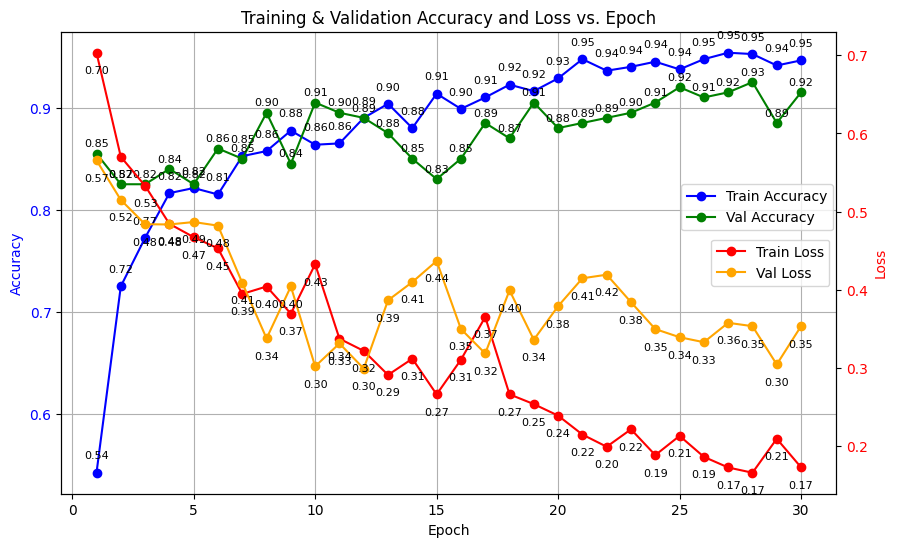
\includegraphics[width=1\textwidth]{Images/acc_loss_vs_epoch.png}
    \caption{Accuracy and Loss versus Epoch in a Single Graph}
    \label{fig:AccLossGraph}
\end{figure}

\noindent From these Figures \ref{fig:AccGraph}, \ref{fig:LossGraph}, \ref{fig:AccLossGraph} it is clear that the model has shown good performance in training, as well as testing. The space between the accuracy curves shows whether the model is overfitting or not, but on keen observation, it is clear that there are no serious signs of overfitting. Also, the troughs and crests are due to the presence of noise and resolution problems of the videos in the dataset.

\clearpage

\subsection{Confusion Matrix}

The Confusion Matrix is a tabular representation of the classification power of the deep learning models. It encodes the values to find other metrics like Precision, Recall, and F1 Score. The confusion matrix of the proposed model is given in Figure \ref{fig:confMatrix}

\begin{figure}[!htbp]
    \centering 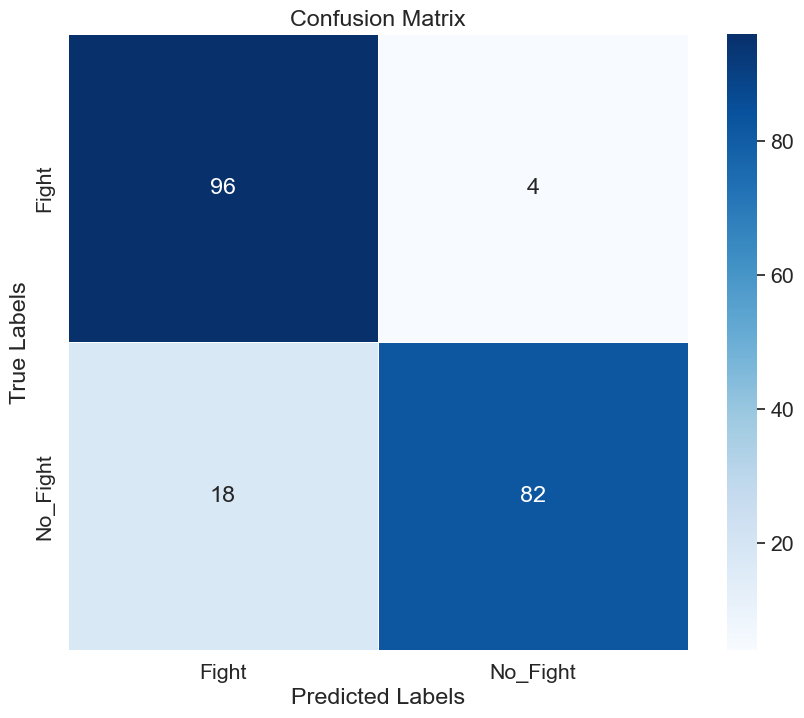
\includegraphics[width=0.65\textwidth]{Images/conf_matrix.png}
    \caption{Confusion Matrix of the Proposed Model}
    \label{fig:confMatrix}
\end{figure}

\noindent Confusion Matrix Analysis:

\begin{enumerate}
    \item True Positive (TP): 96 (Top-left cell) - Correct predictions where the actual class is "Fight" and model predicted, "Fight".

    \item False Positive (FP): 18 (Bottom-left cell) - Times model incorrectly predicted "Fight" when the actual class was "No\_Fight".

    \item False Negative (FN): 4 (Top-right cell) - Times model incorrectly predicted "No\_Fight" when the actual class was "Fight".

    \item True Negative (TN): 82 (Bottom-right cell) - Correct predictions where the actual class is "No\_Fight" and the model also predicted "No\_Fight".
    
\end{enumerate}

\clearpage

\subsection{Accuracy}

\noindent Accuracy is a common performance metric in deep learning, particularly useful for classification problems. It measures the proportion of true results (both true positives and true negatives) to the total observations(true positives, false positives, true negatives, and false negatives). Accuracy is computed as in the general equation \ref{acc},

\begin{equation}
%\[
\text{Accuracy} = \frac{\text{Number of correct predictions}}{\text{Total number of predictions}} = \frac{TP + TN}{TP + TN + FP + FN}
\label{acc}
%\]
\end{equation}

\[
\text{Accuracy (Training/Testing)} = \frac{96 + 82}{96 + 82 + 4 + 18} = \frac{178}{200} = 89\%
\]

% The model shows good accuracy (89\%) and excellent precision for predicting "Fight" (96\%).
% - Recall for "Fight" is lower (84.2\%), indicating room for improvement in capturing all true "Fight" instances.
% - Low number of false positives (4) suggests the model is conservative in predicting "Fight".
% - Adjustments may be necessary based on specific performance goals, especially in terms of sensitivity (recall) for the "Fight" class.

\subsection{Precision}
In violence detection systems, precision is crucial because it measures how many of the detected instances of violence are actually correct. High precision means that when the system identifies an event as violent, there is a high probability that it truly is violent. With high precision, unnecessary panic or resource wastage is minimized. Precision is computed as in the general equation \ref{precision},

\begin{equation}
%\[
\text{Precision} = \frac{TP}{TP + FP}
\label{precision}
%\]
\end{equation}

\[
\text{Precision (Fight)} = \frac{96}{96 + 4} = \frac{96}{100} = 96\%
\]

\[
\text{Precision (No\_Fight)} = \frac{82}{82 + 18} = \frac{82}{100} = 82\%
\]

\subsection{Recall}
Recall is equally critical because it measures the system’s ability to detect all actual violent events captured in the video data. In the context of public safety and security, a high recall rate ensures that no violent incidents go undetected. This is particularly vital in surveillance systems used in public areas like schools, malls, or public transportation, where failing to detect an act of violence can have severe consequences. Recall is computed as in the general equation \ref{recall},

\begin{equation}
%\[
\text{Recall} = \frac{TP}{TP + FN}
\label{recall}
%\]
\end{equation}

\[
\text{Recall (Fight)} = \frac{96}{96 + 18} = \frac{96}{114} \approx 84.2\%
\]

\[
\text{Recall (No\_Fight)} = \frac{82}{82 + 4} = \frac{82}{86} \approx 95.3\%
\]

\subsection{F1 Score}

The F1 score becomes particularly important when balancing the trade-offs between precision and recall. In violence detection, it is often crucial to maintain a balance where both false positives (non-violent acts labeled as violent) and false negatives (violent acts not detected) are minimized. This balance is essential because both types of errors can have serious implications—false positives can lead to unnecessary interventions, while false negatives might allow violent situations to escalate. The F1 score provides a single metric that helps optimize the model during training and tuning to ensure an effective balance between identifying true violence and reporting non-violent activities. Precision is computed as in the general equation \ref{f1score},

\clearpage

\begin{equation}
%\[
F1 = 2 \cdot \frac{\text{Precision} \cdot \text{Recall}}{\text{Precision} + \text{Recall}}
\label{f1score}
%\]
\end{equation}

\[
F1 \text{(Fight)} = 2 \cdot \frac{0.96 \cdot 0.842}{0.96 + 0.842} \approx 89.7\%
\]

\[
F1 \text{ (No\_Fight)} = 2 \cdot \frac{0.82 \cdot 0.953}{0.82 + 0.953} \approx 0.882 \text{ or } 88.2\%
\]

\vspace{1.5cm}

% \begin{minipage}{0.5\textwidth}
% \centering
% \captionof{table}{Training and Testing Metrics}
% \begin{tabular}{c|c|c|c}
% \hline
% \textbf{Criteria} & \textbf{Metric} & \multicolumn{2}{c}{\textbf{Value (\%)}} \\
% \cline{3-4}
%            &                  & \textbf{Training}    & \textbf{Testing} \\ \hline
% Graph     & Accuracy          & 95.00                & 92.00               \\
% Testing   & Accuracy          & 89.00                   & 89.00                \\
% \hline
% \end{tabular}

% \label{table:trainingTestingAccMetric}
% \end{minipage}\hspace{0.03\textwidth}%
% \begin{minipage}{0.5\textwidth}
% \centering
% \captionof{table}{Fight vs No Fight Metrics}
% \begin{tabular}{c|c|c}
% \hline
% \textbf{Metric} & \multicolumn{2}{c}{\textbf{Value (\%)}} \\
% \cline{2-3}
%                 & \textbf{Fight}    & \textbf{No Fight} \\
% \hline
% Precision       & 89.00             & 82                \\
% Recall          & 89.00             & 95.3              \\
% F1-Score        & 88.95             & 88.2              \\
% \hline
% \end{tabular}

% \label{table:otherMetrics}
% \end{minipage}

\begin{table}[!htbp]
\centering
\captionof{table}{Training and Testing Metrics}
\begin{tabular}{c|c|c|c}
\hline
\textbf{Criteria} & \textbf{Metric} & \multicolumn{2}{c}{\textbf{Value (\%)}} \\
\cline{3-4}
           &                  & \textbf{Training}    & \textbf{Testing} \\ \hline
Graph     & Accuracy          & 95.00                & 92.00               \\
Testing   & Accuracy          & 89.00                   & 89.00                \\
\hline
\end{tabular}

\label{table:trainingTestingAccMetric}
\end{table}


\vspace{1.5cm}

\begin{table}[!htbp]
\centering
\captionof{table}{Fight vs No Fight Metrics}
\begin{tabular}{c|c|c}
\hline
\textbf{Metric} & \multicolumn{2}{c}{\textbf{Value (\%)}} \\
\cline{2-3}
                & \textbf{Fight}    & \textbf{No Fight} \\
\hline
Precision       & 96.00             & 82.00                \\
Recall          & 84.20             & 95.30              \\
F1-Score        & 89.70             & 88.20              \\
\hline
\end{tabular}

\label{table:otherMetrics}
\end{table}

\vspace{0.5cm}

\noindent In addition, the overall result values that were computed are written in Table \ref{table:trainingTestingAccMetric} and Table \ref{table:otherMetrics}. The accuracy metrics (given in Table \ref{table:trainingTestingAccMetric}) are different for graph and model testing, this is because of the usage of automatic mechanisms to save the best keras model file based on validation accuracy which is explained in the coding practices section.

\clearpage

\section{Spatial Attention Maps}

Spatial Attention Maps helps to highlight regions of interest within images or data, aiding in the interpretation and understanding of complex visual information. The original image acts as the input, and the spatial attention map overlays above the original image to produce an output as shown in Figure \ref{fig:attmap}.

\begin{figure}[h!]
\centering
\subfloat[Original Image] {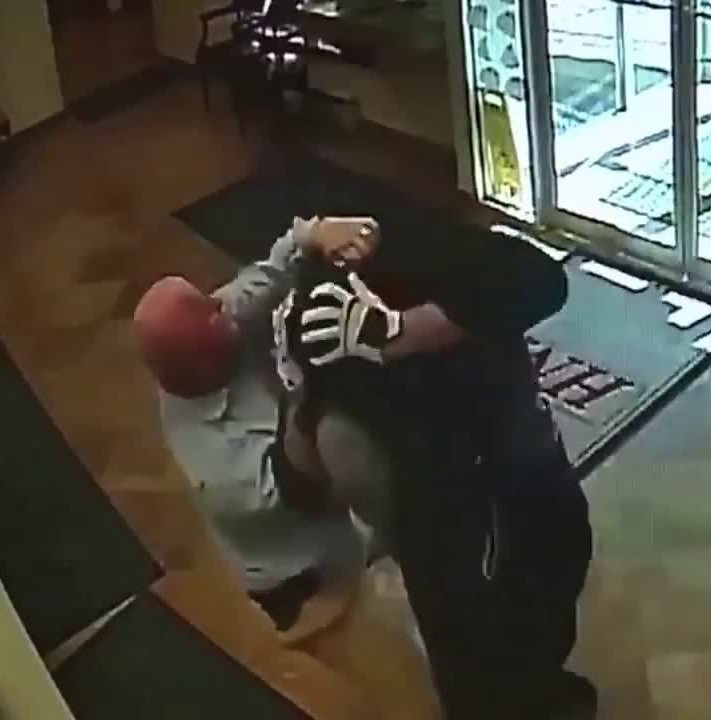
\includegraphics[width=0.3\textwidth]
{Images/attn_maps/1.jpg}}
\hfill
\subfloat[Attention Map] {
\includegraphics[width=0.3\textwidth]
{Images/attn_maps/output.png}}
\hfill
\subfloat[Resultant Attention Map] {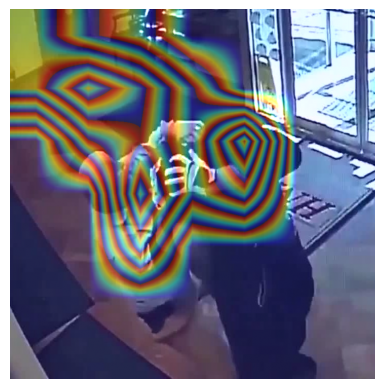
\includegraphics[width=0.3\textwidth]
{Images/attn_maps/1.png}}
\caption{Steps in Generating Attention Map}
\label{fig:attmap}
\end{figure}

\begin{figure}[h!]
\centering
\subfloat[Original Image] {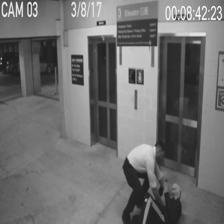
\includegraphics[width=0.45\textwidth]
{Images/attn_maps/2.jpg}}
\hfill
\subfloat[Attention Map] {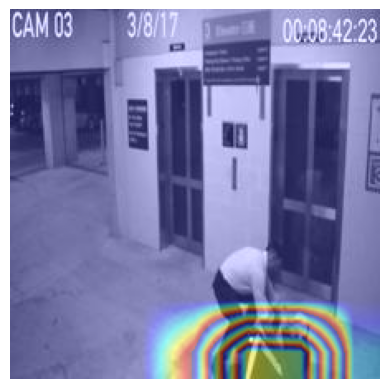
\includegraphics[width=0.45\textwidth]
{Images/attn_maps/2.png}}
\caption{Correct Attention Map}
\label{fig:correctAttn}
\end{figure}

\begin{figure}[h!]
\centering
\subfloat[Original Image] {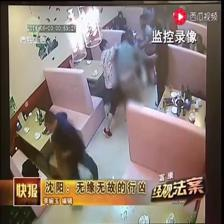
\includegraphics[width=0.45\textwidth]
{Images/attn_maps/4.jpg}}
\hfill
\subfloat[Attention Map] {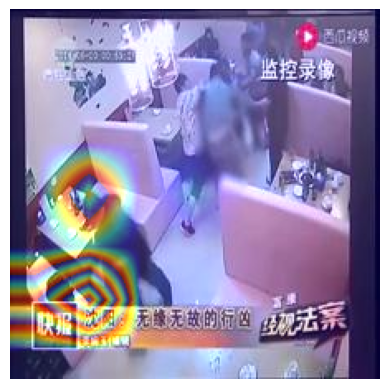
\includegraphics[width=0.45\textwidth]
{Images/attn_maps/4.png}}
\caption{Wrong Attention Map 1}
\label{fig:wrongAttn1}
\end{figure}

\begin{figure}[h!]
\centering
\subfloat[Original Image] {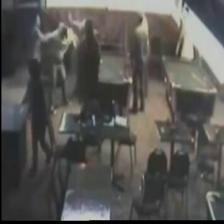
\includegraphics[width=0.45\textwidth]
{Images/attn_maps/5.jpg}}
\hfill
\subfloat[Attention Map] {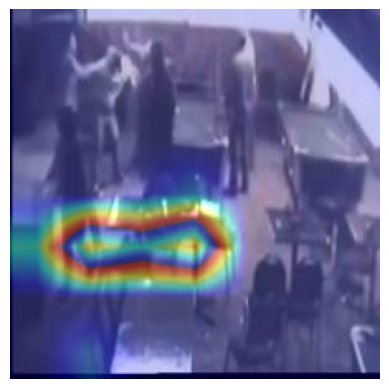
\includegraphics[width=0.45\textwidth]
{Images/attn_maps/5.png}}
\caption{Wrong Attention Map 2}
\label{fig:wrongAttn2}
\end{figure}

\clearpage

\begin{figure}[h!]
\centering
\subfloat[Original Image] {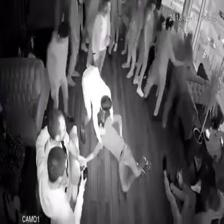
\includegraphics[width=0.325\textwidth]
{Images/attn_maps/7.jpg}}
\hfill
\subfloat[Learning Attention(A)] {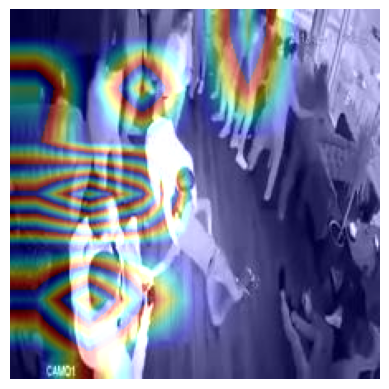
\includegraphics[width=0.325\textwidth]
{Images/attn_maps/7_2.png}}
\hfill
\subfloat[Learning Attention(B)] {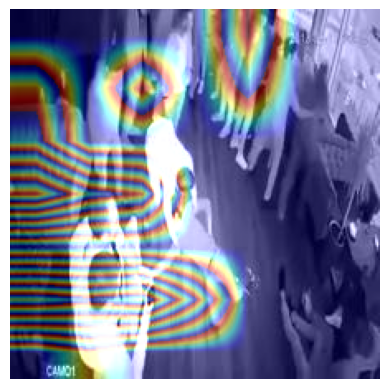
\includegraphics[width=0.325\textwidth]
{Images/attn_maps/7_1.png}}
\caption{Learning Happening in Attention}
\label{fig:learningAttn}
\end{figure}

\begin{itemize}
    \item Purpose: Spatial Attention Maps are used to visually highlight areas within an image that a computational model focuses on when making decisions or predictions. This can help researchers and engineers understand what parts of an image are marked important by the model.

    \item Process: The generated attention map is overlaid on the original images. These maps are color-coded or heat-mapped layers as shown in Figure \ref{fig:attmap}(b) that indicate the `attention` a model gives to different parts of an image when analyzing it. The correct attention map outputs are shown in Figure \ref{fig:correctAttn} and the wrong ones in the \ref{fig:wrongAttn1} and Figure \ref{fig:wrongAttn2}. In addition, Figure \ref{fig:learningAttn} shows how the learning takes place in attention maps over each iteration.

    \item Educational and Diagnostic Use: These attention maps cannot be used for improving the algorithms by tweaking them, but they serve an educational purpose. They can help explain to students and professionals how certain algorithms interpret visual data and what features the network prioritizes. This can be classified as a part of ExplainableAI (XAI)
    
\end{itemize}

\clearpage

\section{Discussions}

\noindent Training a deep learning model without any manual feature engineering to perform well on complex data like real-world fight and violence data is inherently a difficult procedure. In order to make it possible, one way is to make a very deep network with complex architecture that can absorb all the intricacies and nuances in the training data, another way is to do manual feature engineering like annotating the dataset to tell the model where the violence or fight is occurring. Both of these require heavy manual work to make it possible.

\noindent Some of the reasons that fuel the difficulties are that the data were mostly captured from CCTV visuals which has many problems like low resolution, distant and different camera angles views. To make a well-performing and lightweight model(as per the objective) we have to input a lot of data, do validation, and incorporate many precautions to handle edge cases like overfitting, OOM errors, and other problems that are explained in the proposed methodology chapter. But still, the model has managed to overcome these difficulties which were justified by the results of the testing.

\noindent Effectively, the performance metrics like the accuracy-loss graphs and confusion matrix, show insight into the effectiveness and efficiency of our model. Precision shows a measure of the model's exactness by indicating the proportion of positive identifications that were actually correct. Recall provides insight into the model's completeness, reflecting its ability to identify all relevant instances in the dataset. Finally, the F1 Score combines precision and recall into a single metric that captures both the false positives and false negatives. It is particularly useful when the balance between precision and recall is important.

%\begin{figure}
    %\centering
   % \includegraphics[width=0.95\textwidth, height=0.60\textheight]{Activity.jpg.jpeg}
    %\caption{Activity diagram}
%\end{figure}

\lfoot{\textit{Departmant of Artificial Intelligence and Data Science, SJCET Palai}}
\renewcommand{\footrulewidth}{0.4pt}